\documentclass[oneside, 11pt]{article}

\usepackage[T1]{fontenc}
\usepackage[utf8]{inputenc}
\usepackage[dutch]{babel}

\usepackage{fouriernc}
\usepackage[detect-all, load-configurations=binary,
            separate-uncertainty=true, per-mode=symbol,
            retain-explicit-plus, range-phrase={ tot }]{siunitx}

\usepackage{setspace}
\setstretch{1.2}

\setlength{\parskip}{\smallskipamount}
\setlength{\parindent}{0pt}

\usepackage{geometry}
\geometry{marginparwidth=0.5cm, verbose, a4paper, tmargin=3cm, bmargin=3cm, lmargin=2cm, rmargin=2cm}

\usepackage{float}

\usepackage[fleqn]{amsmath}
\numberwithin{equation}{section}
\numberwithin{figure}{section}

\usepackage{graphicx}
\graphicspath{{Figures/}}
\usepackage{subfig}

\usepackage{tikz}
\usetikzlibrary{plotmarks}

\usepackage{fancyhdr}
\pagestyle{fancy}
\fancyhf{}
\rhead{\thepage}
\renewcommand{\footrulewidth}{0pt}
\renewcommand{\headrulewidth}{0pt}

\usepackage{relsize}
\usepackage{xspace}
\usepackage{url}

\newcommand{\figref}[1]{Figuur~\ref{#1}}

\newcommand{\hisparc}{\textsmaller{HiSPARC}\xspace}
\newcommand{\kascade}{\textsmaller{KASCADE}\xspace}
\newcommand{\sapphire}{\textsmaller{SAPPHiRE}\xspace}
\newcommand{\jsparc}{\textsmaller{jSparc}\xspace}
\newcommand{\hdf}{\textsmaller{HDF5}\xspace}
\newcommand{\aires}{\textsmaller{AIRES}\xspace}
\newcommand{\csv}{\textsmaller{CSV}\xspace}
\newcommand{\python}{\textsmaller{PYTHON}\xspace}
\newcommand{\corsika}{\textsmaller{CORSIKA}\xspace}
\newcommand{\labview}{\textsmaller{LabVIEW}\xspace}
\newcommand{\daq}{\textsmaller{DAQ}\xspace}
\newcommand{\adc}{\textsmaller{ADC}\xspace}
\newcommand{\adcs}{\textsmaller{ADC}s\xspace}
\newcommand{\Adcs}{A\textsmaller{DC}s\xspace}
\newcommand{\hi}{\textsc{h i}\xspace}
\newcommand{\hii}{\textsc{h ii}\xspace}
\newcommand{\mip}{\textsmaller{MIP}\xspace}
\newcommand{\hisparcii}{\textsmaller{HiSPARC II}\xspace}
\newcommand{\hisparciii}{\textsmaller{HiSPARC III}\xspace}
\newcommand{\pmt}{\textsmaller{PMT}\xspace}
\newcommand{\pmts}{\textsmaller{PMT}s\xspace}

\DeclareSIUnit{\electronvolt}{\ensuremath{\mathrm{e\!\!\:V}}}

\DeclareSIUnit{\unitsigma}{\ensuremath{\sigma}}
\DeclareSIUnit{\mip}{\textsmaller{MIP}}
\DeclareSIUnit{\adc}{\textsmaller{ADC}}

\DeclareSIUnit{\gauss}{G}
\DeclareSIUnit{\parsec}{pc}
\DeclareSIUnit{\year}{yr}


\newcolumntype{x}[1]{>{\centering\arraybackslash\hspace{0pt}}p{#1}}

\title{Air-showers, events en coïncidenties}
\author{N.G. Schultheiss}
\docwerkblad{1}{AS}
\version{1.2}

\begin{document}

\maketitle

\section{Inleiding}

Kosmische deeltjes bestaan uit snel bewegende atoomkernen, neutrino's
of gamma fotonen. Deze primaire kosmische deeltje hebben voldoende
energie om interacties aan te gaan met deeltjes in de atmosfeer%
\footnote{Achtergronden over deze interacties zijn op RouteNet te vinden in
de modules ,,Deeltjes in het standaardmodel'' en ,,Krachten in
het standaard model''. (\url{http://www.hisparc.nl/docent-student/lesmateriaal/routenet/})%
}. Ten gevolge van deze interacties ontstaan grote aantallen nieuwe deeltjes, voornamelijk pionen, die na korte tijd vervallen
weer naar muonen en elektronen en hun antideeltjes of gamma fotonen.
Een gamma foton kan worden omgezet in een paar van een elektron en een positron (een
anti-elektron). Bij de interactie tussen een positron
en een elektron verdwijnen de deeltjes en wordt de vrijkomende energie
in twee nieuwe gamma fotonen omgezet. Als geladen deeltjes worden
afgebogen ontstaan er ook (gamma) fotonen. Deze processen gaan door
totdat de energie te laag is voor de creatie van een elektron / positron
paar.

Een enkel kosmisch deeltje met voldoende energie start dus een lawine
van deeltjes in de atmosfeer, de air-shower. Als de energie van de air-shower groot genoeg is, kunnen grote hoeveelheden deeltjes de grond bereiken en een signaal afgeven in een detector. De grote
hoeveelheid deeltjes maakt een statistische interpretatie van de metingen
mogelijk.


\section{Events}

Wanneer bij een air-shower enorme hoeveelheden deeltjes de grond bereiken,
kunnen we vaststellen of er een kosmisch deeltje in de atmosfeer is binnengedrongen.
Meerdere detectoren van een station meten in dat geval nagenoeg tegelijk iets, dit
wordt een \emph{event} genoemd. Een enkele detector op de grond
kan naast deeltjes van een air-shower ook de straling meten van radioactief
verval van stoffen op Aarde, een dergelijke meting wordt een \emph{single}
genoemd.

\begin{figure}[ht]
    \centering
    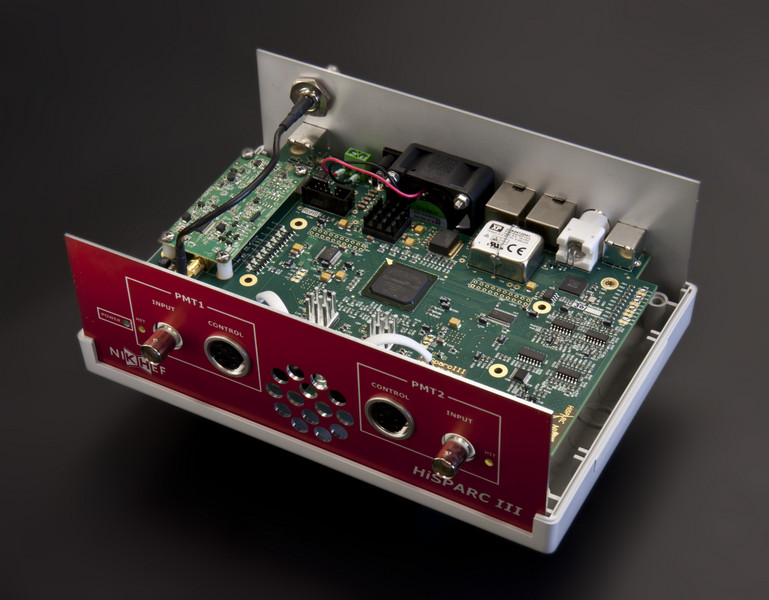
\includegraphics[scale=1.5]{8cee5cc97a}
    \caption{De HiSPARC master unit, foto uit \cite{nikhefhisparc}. In de
             blokken PMT 1 en PMT 2 zijn twee gele ledjes te zien. Deze
             lichten op als er deeltjes door respectievelijk detector 1
             of detector 2 wordt gemeten. In de praktijk worden de
             detectoren ongeveer elke \SI{10}{\milli\second} geraakt.
             Achter de koelgaten is een witte led te zien. Deze licht op
             als beide detectoren binnen een tijdsinterval van
             \SI{1.5}{\micro\second} deeltjes waarnemen, dit komt veel
             minder vaak voor.}
\end{figure}


\subsection{De nauwkeurigheid van het meten van events}

Een \emph{event} vindt plaats als het station getriggerd wordt.
Bij een tweeplaatsstation wordt het station getriggerd als beide detectoren
binnen \SI{1,5}{\micro\second} een signaal lager dan \SI{-70}{\milli\volt}
afgeven. Een vierplaatsstation wordt ook getriggerd als drie detectoren
binnen \SI{1,5}{\micro\second} een signaal lager dan \SI{-30}{\milli\volt}
afgeven. Als het station getriggerd wordt, licht er een witte led
achter de koelgaten van het HiSPARC kastje op. De tijd van het event
is de tijd waarop aan de triggervoorwaarde is voldaan, dit is dus
de tweede of derde tijd van een single.

\begin{minipage}[t]{1\columnwidth}%

\paragraph{Opdracht 1:}

Bepaal hoe vaak het witte ledje in 1 minuut oplicht. Doe dit 5 keer
en vul de resultaten in de tabel op de volgende pagina in.
Gebruik als je geen \hisparc kastje hebt de volgende website om het
meten van een event te simuleren.\\
\url{http://data.hisparc.nl/media/jsparc/trigger_simulation.html}


\vspace{1em}
\begin{tabular}{|x{.11\textwidth}|x{.11\textwidth}|x{.11\textwidth}
                |x{.11\textwidth}|x{.11\textwidth}|x{.11\textwidth}
                |x{.11\textwidth}|}
    \cline{2-7}
    \multicolumn{1}{c|}{} & 1 & 2 & 3 & 4 & 5 & $N_\textrm{gem}$\\
    \hline
    $N$ &  &  &  &  &  & \tabularnewline
    \hline
\end{tabular}%
\end{minipage}

\bigskip{}

\begin{minipage}[t]{1\columnwidth}%

\paragraph{Opdracht 2:}

Bepaal naast het gemiddelde ook de maximale en de minimale
waarde. Leg uit welke nauwkeurigheid je verwacht.

\begin{center}
    \rule{\textwidth}{0.3mm}\\
    \rule{\textwidth}{0.3mm}\\
    \rule{\textwidth}{0.3mm}\\
    \rule{\textwidth}{0.3mm}\\
\end{center}
\end{minipage}

\bigskip{}


De nauwkeurigheid is ook wiskundig te bepalen. daartoe gaan we de spreiding $\sigma$ uitrekenen.

\begin{minipage}[t]{1\columnwidth}%

\paragraph{Opdracht 3:}

Bereken het gemiddelde van $N^{2}$.

\bigskip{}


\begin{tabular}{|x{.11\textwidth}|x{.11\textwidth}|x{.11\textwidth}
                |x{.11\textwidth}|x{.11\textwidth}|x{.11\textwidth}
                |x{.11\textwidth}|}
    \cline{2-7}
    \multicolumn{1}{c|}{} & 1 & 2 & 3 & 4 & 5 & $\left(N^{2}\right)_\textrm{gem}$\\
    \hline
    $N^{2}$ &  &  &  &  &  & \\
    \hline
\end{tabular}

\bigskip{}

De spreiding is nu te berekenen met
$\sigma=\sqrt{\left(N^{2}\right)_\textrm{gem}-\left(N_\textrm{gem}\right)^{2}}$ dit is
dus de wortel uit het gemiddelde van de kwadraten min het kwadraat van
het gemiddelde ($N_\textrm{gem}$ is al in opdracht 1 berekend).

\end{minipage}

\bigskip{}


\begin{minipage}[t]{1\columnwidth}%

\paragraph{Opdracht 4:}

Welke conclusie mag je trekken als je de waarden die je bij
opdracht 2 en 3 hebt gevonden vergelijkt?

\begin{center}
    \rule{\textwidth}{0.3mm}\\
    \rule{\textwidth}{0.3mm}\\
    \rule{\textwidth}{0.3mm}\\
    \rule{\textwidth}{0.3mm}\\
\end{center}
\end{minipage}


\subsection{Het toetsen van de hypothese}

Het signaal van een enkele detector -een single- wordt gezien als
achtergrondstraling. De gelijktijdige signalen van twee detectoren
-een event- wijzen op een air-shower. Beide delen van de hypothese
zijn natuurlijk te onderzoeken.


\subsubsection{Het signaal van een enkele detector wordt gezien als achtergrondstraling.}

Hoe groot is de kans dat het station wordt getriggerd door achtergrondstraling?
De detector geeft alleen een signaal af als er een deeltje door de
detector gaat. Om van een air-shower te spreken moeten de deeltjes
binnen een triggervenster van \SI{1.5}{\micro\second} gedetecteerd
worden. De achtergrondstraling zorgt dat gemiddeld ongeveer elke
10 ms een deeltje door een detector van \SI{0.500}{\meter} bij \SI{1.000}{\meter}
schiet%
\footnote{Als er op school een Geigerteller is, kan de achtergrondstraling in
$\mathrm{\left[pulsen/s/m^{2}\right]}$ ook worden gemeten. Naast
het aantal pulsen per seconde is dus ook het oppervlak van de detector
van belang.%
}. Als deze singles netjes verdeeld zouden zijn, is de kans op een
tweede toevallig gemeten deeltje van de achtergrondstraling binnen
het triggervenster van \SI{1.5}{\micro\second} te berekenen.

\begin{minipage}[t]{1\columnwidth}%

\paragraph{Opdracht 5:}

Bereken (met een boxplot) hoe groot de kans is dat er een
tweede radioactief verval binnen \SI{1.5}{\micro\second} van de eerste
radioactief verval optreedt.

\begin{center}
    \rule{\textwidth}{0.3mm}\\
    \rule{\textwidth}{0.3mm}\\
    \rule{\textwidth}{0.3mm}\\
    \rule{\textwidth}{0.3mm}\\
\end{center}
\end{minipage}

\bigskip{}

Een nettere manier om deze kans te berekenen is in 1838 door Siméon
Poisson \cite{wiki} gepubliceerd:

\begin{equation}
    P_{k}=\frac{\lambda^{k}}{k!}e^{-\lambda}
\end{equation}

Hierin is $k=1$ als een tweede detector precies éénmaal getriggerd
wordt. $\lambda$ is hier de frequentie van de achtergrondstraling
maal de duur van het triggervenster $\left(\lambda=f_{single}*T_\textrm{venster}\right)$.

\begin{minipage}[t]{1\columnwidth}%

\paragraph{Opdracht 6:}

Laat zien dat de met de boxplot berekende waarde nauwelijks
afwijkt van de met de Poisson-formule berekende waarde $P_{k=1}$.

\begin{center}
    \rule{\textwidth}{0.3mm}\\
    \rule{\textwidth}{0.3mm}\\
    \rule{\textwidth}{0.3mm}\\
    \rule{\textwidth}{0.3mm}\\
\end{center}
\end{minipage}

\bigskip{}

Eventueel geldt bij een toevallige trigger ook $k=2$, $k=3$ etc.
In het algemeen nemen we $k>0$ (met $k\mathbb{\in N}$). De kans
dat er GEEN toevallige trigger optreedt is $P_{k=0}$.

\begin{minipage}[t]{1\columnwidth}%

\paragraph{Opdracht 7:}

Met de kans dat er geen toevallige trigger optreed, is de
kans op een toevallige trigger ook te berekenen. (De kans op een trigger
plus de kans op geen trigger is 100\%.) Bereken deze kans.

\begin{center}
    \rule{\textwidth}{0.3mm}\\
    \rule{\textwidth}{0.3mm}\\
    \rule{\textwidth}{0.3mm}\\
    \rule{\textwidth}{0.3mm}\\
\end{center}
\end{minipage}

\bigskip{}

De duur van het triggervenster is van belang als we naar de kans op
toevallige triggers kijken. We kunnen een grafiek maken van de kans
op een toevallige trigger als functie van de duur van het triggervenster
$T_\textrm{venster}$. Er geldt: $\lambda=f_{single}*T_\textrm{venster}$, en dit
geval wordt dit: $\lambda=100*T_\textrm{venster}$$ $.

\begin{minipage}[t]{1\columnwidth}%

\paragraph{Opdracht 8:}

Maak de onderstaande tabel voor een station met twee detectoren
af.

\bigskip{}


\begin{tabular}{|x{.20\textwidth}|x{.07\textwidth}|x{.07\textwidth}
                |x{.07\textwidth}|x{.07\textwidth}|x{.07\textwidth}
                |x{.07\textwidth}|x{.07\textwidth}|}
    \hline
    $T_\textrm{venster}$ {[}$\mu\mathrm{s}${]} & 1,5 & 3,0 & 7,5 & 15 & 30 & 75 & 150\tabularnewline
    \hline
    $P_\textrm{trigger}=1-P_{k=0}$ &  &  &  &  &  &  & \tabularnewline
    \hline
\end{tabular}
\end{minipage}

\bigskip{}


\begin{figure}[ht]
    \paragraph{Opdracht 9:}

    Maak het diagram van de kans op een toevallige trigger als
    functie van de duur van het triggervenster.\bigskip{}

    
\begin{tikzpicture}
        [gridlines/.style={color=gray,very thin}]
        \draw [gridlines, step=.5cm] (0,0) grid (\textwidth,8cm);
    \end{tikzpicture}
\end{figure}

\bigskip{}

Tot nu toe zijn we uitgegaan van een station met twee detectoren.
Bij een station met vier detectoren zijn er logischerwijs twee detectoren
meer.

\begin{minipage}[t]{1\columnwidth}%

\paragraph{Opdracht 10:}

Beredeneer hoe groot de kans op een toevallige trigger is
bij een station met 4 detectoren en een triggervenster van \SI{1.5}{\micro\second}
(Denk aan het aantal mogelijke combinaties!).

\begin{center}
    \rule{\textwidth}{0.3mm}\\
    \rule{\textwidth}{0.3mm}\\
    \rule{\textwidth}{0.3mm}\\
    \rule{\textwidth}{0.3mm}\\
\end{center}
\end{minipage}

\bigskip{}

\subsubsection{De gelijktijdige signalen van twee detectoren wijzen op
               een air-shower.}

Dit experiment is uit te voeren met de simulatie op (figuur \ref{fig:Station_simulatie}):

\url{http://data.hisparc.nl/media/jsparc/station_simulation.html}

\begin{figure}[H]
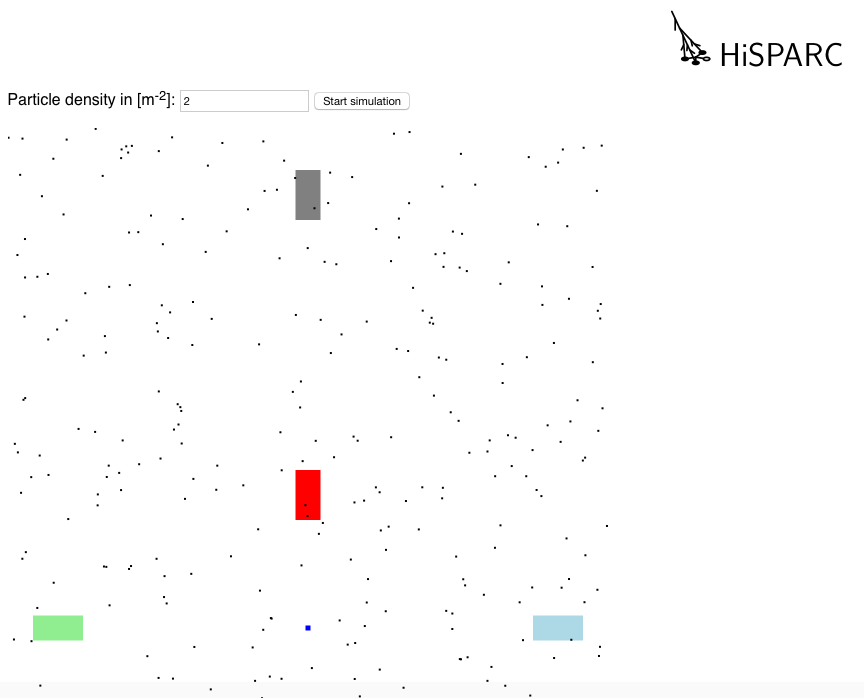
\includegraphics[width=15cm]{Station_simulation}

\caption{\label{fig:Station_simulatie}Station simulatie. Het aantal deeltjes
per m$^{2}$ in een deeltjes-lawine kan worden ingevuld. In dit geval zijn er
dus gemiddeld 2 deeltjes per m$^{2}$. Met de knop 'Start simulation' zijn deze
willekeurig te verstrooien. We nemen aan dat het station getriggerd wordt als
minimaal twee detectoren door een deeltje geraakt worden}

\end{figure}


De simulatie gaat verder bij opdracht 14.

Deze simulatie is ook met een practicum te simuleren. In
figuur \ref{fig:Meetstations} is een plattegrond te zien. Hierop
zijn zowel een station met 2 detectoren als een station met 4 detectoren
te zien. De plattegrond past in de deksel van een papierdoos. Op de
plattegrond zijn de scintillatorplaten van \SI{0.500}{\meter} bij
\SI{1.000}{\meter} op schaal getekend.

\begin{figure}[h]
    \centering
    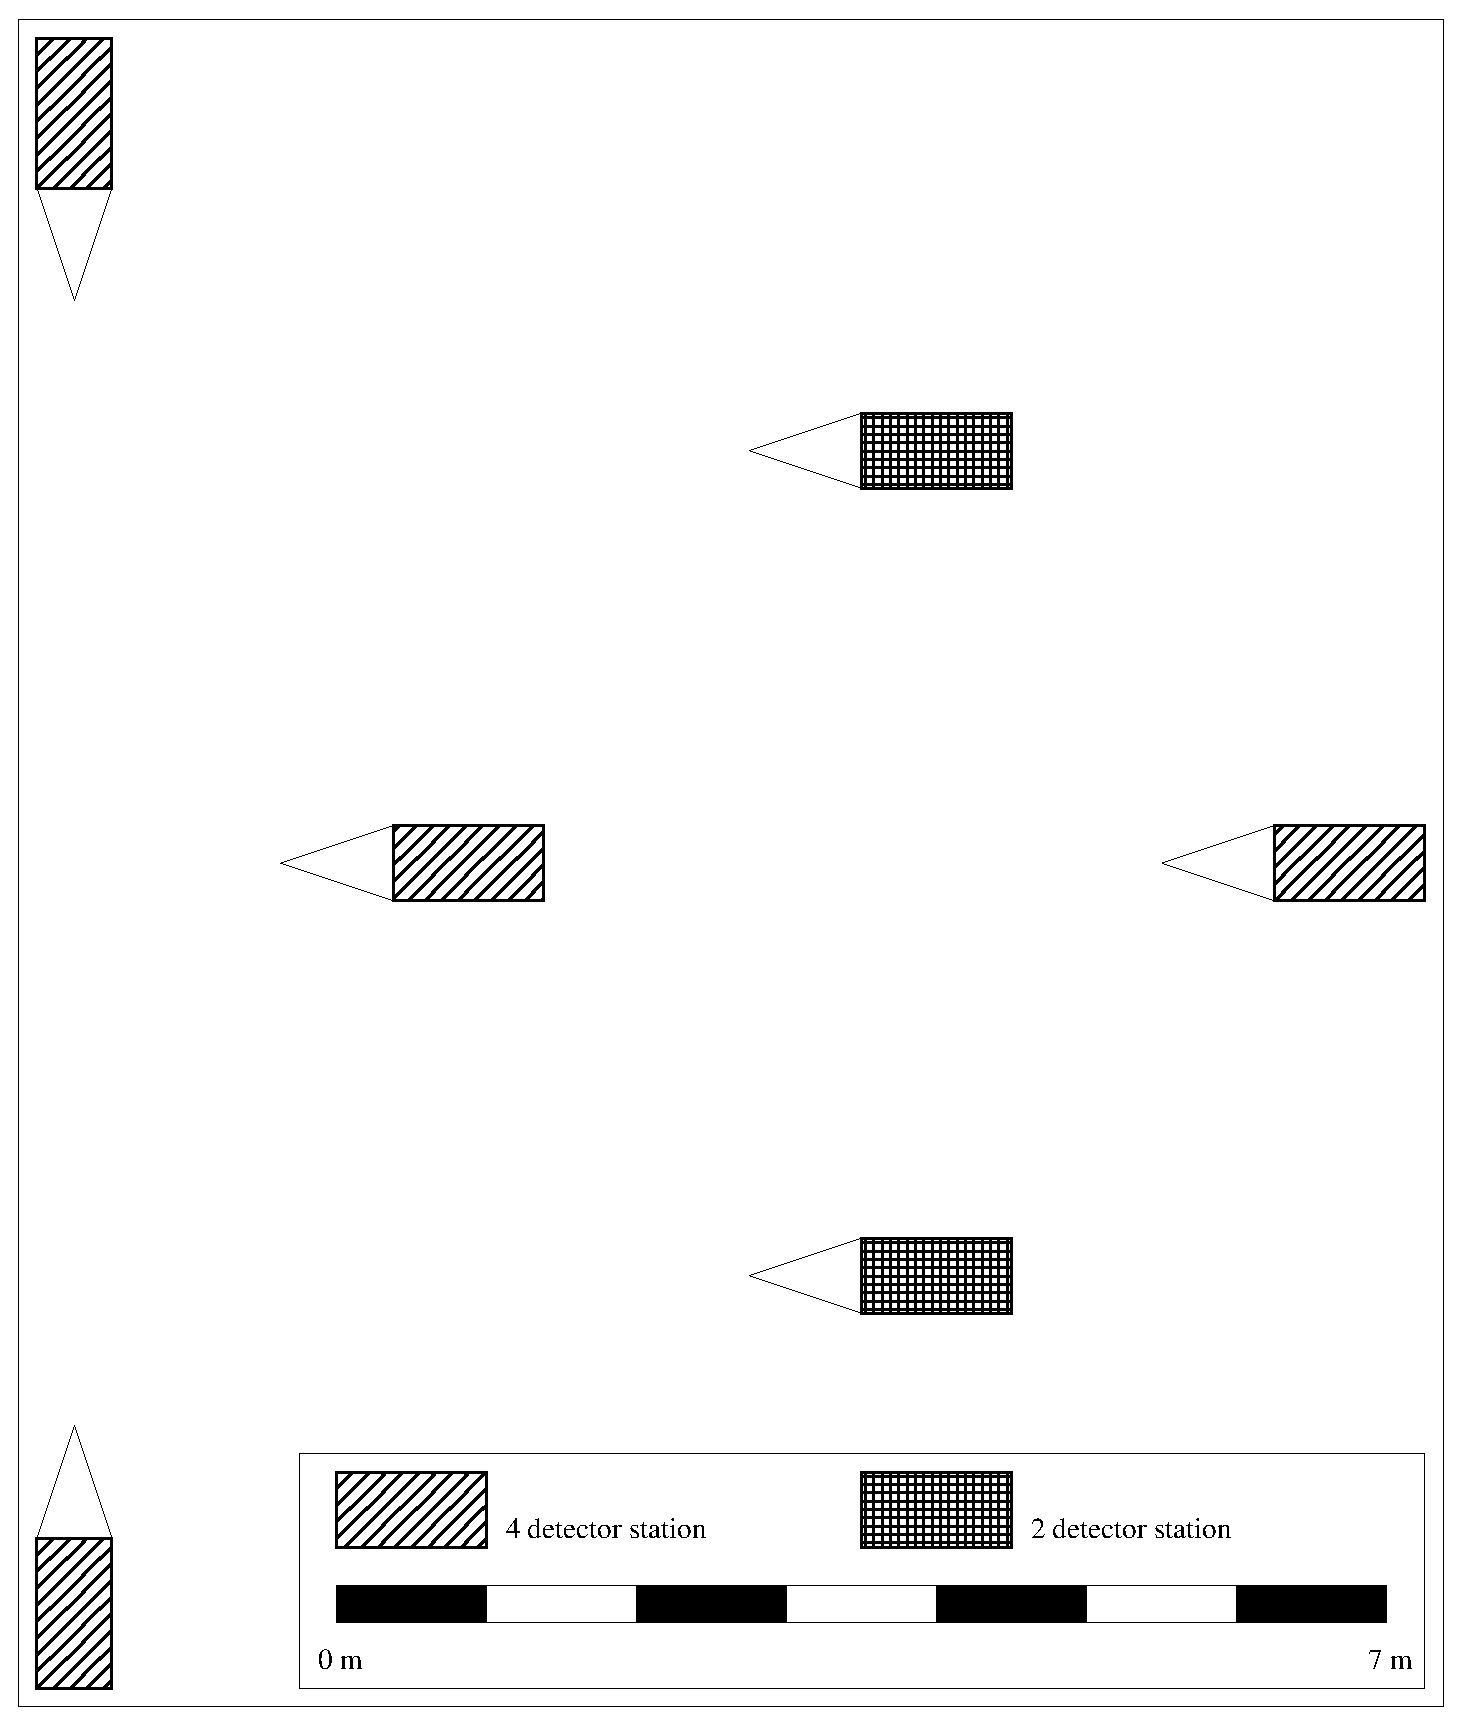
\includegraphics[width=15.833cm]{station}
    \caption{Een meetstation met twee detectoren en een
    meetstation met vier detectoren.}
    \label{fig:Meetstations}
\end{figure}

\begin{minipage}[t]{\columnwidth}%

\paragraph{Opdracht 11:}

Bepaal het oppervlak in de doos in $\mathrm{cm^{2}}$. In
werkelijkheid komt dit overeen met een oppervlak in $\mathrm{m^{2}}$,
dit tweede oppervlak is te berekenen.

\begin{center}
    \rule{\textwidth}{0.3mm}\\
    \rule{\textwidth}{0.3mm}\\
    \rule{\textwidth}{0.3mm}\\
    \rule{\textwidth}{0.3mm}\\
\end{center}
\end{minipage}\bigskip{}

We willen de kans bepalen dat een air-shower gedetecteerd wordt. Deze
kans hangt af van de deeltjesdichtheid $\rho$, het aantal deeltjes
per $\mathrm{m^{2}}$ in de air-shower. Deze deeltjes simuleren we
met korreltjes risotto of parel couscous. Hier gaan we met risotto aan de slag.

\begin{minipage}[t]{1\columnwidth}%

\paragraph{Opdracht 12:}

Bereken hoeveel deeltjes nodig zijn.

\bigskip{}

\begin{tabular}{|x{.3\textwidth}|x{.1\textwidth}|x{.1\textwidth}
                |x{.1\textwidth}|x{.1\textwidth}|x{.1\textwidth}|}
    \hline
    $\rho_\textrm{werkelijk}$ $\left[\mathrm{m^{-2}}\right]$ & 0,5 & 1 & 2 & 5 & 10 \\
    \hline
    Aantal korreltjes in de doos &  &  &  &  & \\
    \hline
    \end{tabular}%
\end{minipage}

\bigskip{}
Het wordt een heel karwei om de korreltjes te tellen. We wegen een
aantal korreltjes en bereken de massa risotto die nodig is.

\begin{minipage}[t]{1\columnwidth}%

\paragraph{Opdracht 13:}

Bereken de massa risotto.

\bigskip{}

\begin{tabular}{|x{.3\textwidth}|x{.1\textwidth}|x{.1\textwidth}
                |x{.1\textwidth}|x{.1\textwidth}|x{.1\textwidth}|}
    \hline
    $\rho_\textrm{werkelijk}$ $\left[\mathrm{m^{-2}}\right]$ & 0,5 & 1 & 2 & 5 & 10 \\
    \hline
    Massa risotto in de doos &  &  &  &  & \\
    \hline
\end{tabular}
\end{minipage}

\bigskip{}


Nu kunnen we de hoeveelheid risotto in de doos doen die overeenkomt met
0,5 deeltjes per $\mathrm{m^{2}}$ in werkelijkheid. We schudden de doos
en proberen de risotto zo gelijkmatig te verdelen. Als er op twee
detectoren van een station minstens 1 korreltje ligt is het station
getriggerd. Let op dat je niet elke keer net zo lang schudt totdat er ,,toevallig''
een trigger wordt afgegeven. Dit is een aantal malen te herhalen en we
kunnen aanvinken of het ,,station'' getriggerd wordt of niet. Let op,
één detector kan per keer maximaal een tiental deeltjes meten.

\begin{minipage}[t]{1\columnwidth}

\paragraph{Opdracht 14:}

Voer het experiment een aantal keren uit en bepaal de kans
dat het station getriggerd wordt.

\bigskip{}


\begin{tabular}{|>{\centering}p{2.2cm}|>{\centering}p{1cm}|>{\centering}p{1cm}
                |>{\centering}p{1cm}|>{\centering}p{1cm}|>{\centering}p{1cm}
                |>{\centering}p{1cm}|>{\centering}p{1cm}|>{\centering}p{1cm}
                |>{\centering}p{1cm}|>{\centering}p{1cm}|}
    \cline{2-11}
    \multicolumn{1}{c|}{} & \multicolumn{5}{c|}{twee detectoren} & \multicolumn{5}{c|}{vier detectoren}\tabularnewline
    \hline
    $\rho$ $\left[\mathrm{m^{-2}}\right]$ & 0,5 & 1 & 2 & 5 & 10 & 0,5 & 1 & 2 & 5 & 10\tabularnewline
    \hline
    meting 1 &  &  &  &  &  &  &  &  &  & \tabularnewline
    \hline
    meting 2 &  &  &  &  &  &  &  &  &  & \tabularnewline
    \hline
    meting 3 &  &  &  &  &  &  &  &  &  & \tabularnewline
    \hline
    meting 4 &  &  &  &  &  &  &  &  &  & \tabularnewline
    \hline
    meting 5 &  &  &  &  &  &  &  &  &  & \tabularnewline
    \hline
    meting 6 &  &  &  &  &  &  &  &  &  & \tabularnewline
    \hline
    meting 7 &  &  &  &  &  &  &  &  &  & \tabularnewline
    \hline
    meting 8 &  &  &  &  &  &  &  &  &  & \tabularnewline
    \hline
    meting 9 &  &  &  &  &  &  &  &  &  & \tabularnewline
    \hline
    meting 10 &  &  &  &  &  &  &  &  &  & \tabularnewline
    \hline
    triggerkans &  &  &  &  &  &  &  &  &  & \tabularnewline
    \hline
\end{tabular}
\end{minipage}

\bigskip{}


Met deze gegevens is een diagram voor de triggerkans als functie van
de deeltjesdichtheid te maken.

\begin{figure}[h]
    \paragraph{Opdracht 15:}
    	Maak het diagram van de triggerkans als functie van de
         deeltjesdichtheid, voor een station met twee en een station
         met vier detectoren.

    \bigskip{}
    
\begin{tikzpicture}
        [gridlines/.style={color=gray,very thin}]
        \draw [gridlines, step=.5cm] (0,0) grid (\textwidth,8cm);
    \end{tikzpicture}
    \bigskip{}

    \caption{Het diagram van de triggerkans als functie van de deeltjesdichtheid $\rho$.}
\end{figure}


\section{Coïncidenties}

Een event vindt plaats als twee of meerdere detectoren van een station
nagenoeg tegelijkertijd worden getriggerd. Dit gebeurt al met relatief
kleine air-showers. Een grotere air-shower%
\footnote{De grote van de voetafdruk van de air-shower op Aarde is een maat
voor de hoeveelheid energie van het primaire kosmische deeltje dat
als eerste de atmosfeer raakt.%
} kan deeltjes over een groter oppervlak verspreiden. In dit grotere
oppervlak kunnen meerdere stations liggen. Als meerdere stations nagenoeg
tegelijk worden getriggerd, spreken we van een coïncidentie.

Als een coïncidentie door een enkele air-shower wordt veroorzaakt,
moeten de metingen aan een aantal randvoorwaarden voldoen. Deeltjes
kunnen niet sneller dan de lichtsnelheid bewegen. De locaties van
de stations zijn bekend. Als een station getriggerd wordt, wordt deze
tijd binnen het station op \SI{2.5}{\nano\second} nauwkeurig opgeslagen.
Tussen stations onderling geldt een nauwkeurigheid van \SI{15}{\nano\second}.
Omdat de afstand tussen de stations bekend is, is er een vrij klein
tijdvenster waarbinnen de detectoren deeltjes kunnen meten. Met de
afstanden tussen de stations en de triggertijden is het zelfs mogelijk
om de richting van de air-shower te bepalen \cite{veen2013richting}.

\bigskip{}


\begin{minipage}[t]{1\columnwidth}%

\paragraph{Opdracht 16}

Ook bij coïncidenties kan een triggervenster worden gebruikt.
Dit venster hangt af van de afstand tussen de stations en de lichtsnelheid.
De air-shower geeft het grootste tijdverschil als deze horizontaal
door de opstelling beweegt. Een dergelijke air-shower wordt gegenereerd
door een primair kosmisch deeltje met een extreem grote energie. In
de praktijk komen deze air-showers zelden voor.

Bereken de grootte van het triggervenster in de volgende gevallen:

\bigskip{}

\begin{tabular}{|c|>{\centering}p{1.5cm}|>{\centering}p{1.5cm}|>{\centering}p{1.5cm}|>{\centering}p{1.5cm}|}
    \hline
    Afstand tussen de stations {[}m{]} & 100 & 200 & 500 & 1000\tabularnewline
    \hline
    Duur van het triggervenster {[}ns{]} &  &  &  & \tabularnewline
    \hline
\end{tabular}%
\end{minipage}


\subsection{Tijdsverschillen tussen stations}

De gemeten tijd van de verschillende stations heeft een nauwkeurigheid
van \SI{15}{\nano\second}. Als we uitgaan van de hypothese dat de
kosmische straling in dezelfde mate vanuit elk punt aan de hemel
komt en de klokken allemaal goed lopen, zal het gemiddelde tijdsverschil
bij een voldoende grote steekproef \SI{0}{\nano\second} moeten zijn.
Als er een tijdsverschil gemeten wordt, lopen de klokken niet synchroon.
We kunnen zelfs bepalen hoeveel de klokken voor of achter lopen. Dit
kan door gebruik te maken van event gegevens van een aantal stations.

Deze zijn bijvoorbeeld op te vragen met:

\url{http://data.hisparc.nl/data/501/events?start=2013-08-01+00:00:00&end=2013-08-01+01:00:00}.

Het stationnummer (501), het startmoment (datum (2013-08-01) en tijd
(00:00:00)) en het stopmoment (datum (2013-08-01) en tijd (01:00:00))
worden in de url%
\footnote{Unified Resource Locator: het internet adres.%
} meegestuurd, hier zijn ook andere stationnummers, data en tijden
in te vullen%
\footnote{In principe kan een grote periode worden opgevraagd. Begin echter
met een uur, het opvragen van een dag voor meerdere stations duurt
wel even.%
}. De server stuurt een tsv%
\footnote{Tab-seperated-values: een format waarbij de waarden door tabs gescheiden zijn.%
}-bestand met event gegevens terug. Dit bestand is in een spreadsheet
programma te openen, maar kan ook door JavaScript worden ingelezen.

Om de verschiltijden te bepalen kan de volgende procedure gevolgd
worden:
\begin{itemize}
    \item Geef de stations namen, bijvoorbeeld a, b, c, etc.
    \item Neem de eerste tijd van station a en kijk of er binnen het
    venster events van de stations b, c, etc. zijn. Schrijf de
    tijdverschillen van a met b, c, etc. op en verwijder de eerste tijd
    uit de lijst van station a.
    \item Neem de eerste tijd van station b en kijk of er binnen het
    venster events van de stations c, etc. zijn. Schrijf de
    tijdverschillen van b met c, etc. op en verwijder de eerste tijd uit
    de lijst van station b.
    \item Herhaal dit tot het een na laatste station.
    \item Begin opnieuw bij station a met de kortere lijst en herhaal
    alles tot de lijsten leeg zijn.
    \item We hebben nu verschillijsten van a en b, a en c, etc. Er zijn
    ook verschillijsten van b en c, etc. Met deze lijsten zijn
    histogrammen te maken.
\end{itemize}
We weten dat stations niet nauwkeuriger kunnen meten dan
\SI{2,5}{\nano\second}. Karl Pearson (1857-1936) \cite{wiki} ontwikkelde
een methode om met lijsten gebeurtenissen een histogram te maken. In dit
geval gaan we uit van het aantal verschiltijden (de frequentie van
verschiltijden) tussen twee grenzen (de bin-waarden). Een reeks grenzen
levert een reeks frequenties op. Hiermee is een histogram of
staafdiagram te maken. We kunnen de grenzen bijvoorbeeld zo vastleggen:

\bigskip{}
\begin{tabular}{|c|c|c|c|c|c|c|c|c|}
    \hline
    Bin-waarde {[}ns{]} & eerder & -7,5 tot -5 & -5 tot -2,5 & -2,5 tot 0 & 0 tot 2,5 & 2,5 tot 5 & 5 tot 7,5 & later\tabularnewline
    \hline
    Frequentie &  &  &  &  &  &  &  & \tabularnewline
    \hline
\end{tabular}

\bigskip{}

Het maken van een dergelijke tabel is een behoorlijke klus met een
spreadsheet programma. Het uiteindelijke histogram is langs de horizontale
as te verdelen in bin-waarden. Langs de verticale as komen de frequenties
te staan. In het ideale geval ligt het maximum bij \SI{0}{\nano\second}.
In de praktijk zal dit zelden het geval zijn.

\bigskip{}


\begin{minipage}[t]{1\columnwidth}

\paragraph{Opdracht 17}

\textit{Het bepalen van de bin-breedte -de afstand tussen de bin-waarden-
verdient enige aandacht. Als de frequentie van verschilwaarden laag
is, is het niet handig om een kleine bin-breedte te nemen. De frequentie
hangt namelijk af van de bin-breedte. Een kleine bin-breedte geeft
een grote nauwkeurigheid in de tijd, maar een lage frequentie. Een
grote bin-breedte geeft een hoge frequentie maar een kleine nauwkeurigheid
in de tijd.}

\textit{Bedenk een methode om de bin-breedte handig te kiezen als
het totale aantal verschiltijden (coïncidenties) (N) en de minimale
($t_\textrm{min}$) en maximale ($t_\textrm{max}$) bin-waarde bekend zijn:}

\begin{center}
    \rule{\textwidth}{0.3mm}\\
    \rule{\textwidth}{0.3mm}\\
    \rule{\textwidth}{0.3mm}\\
    \rule{\textwidth}{0.3mm}\\
\end{center}
\end{minipage}


\begin{thebibliography}{9}
    \bibitem{nikhefhisparc} Nikhef, \emph{\hisparc Elektronica},\\
    \url{https://www.nikhef.nl/wetenschap-techniek/technische-afdelingen/
	  elektronicatechnologie/projecten/}.

    \bibitem{wiki} Wikipedia, \\
    \url{http://www.wikipedia.org}.

    \bibitem{veen2013richting} C.G.N. van Veen, \emph{Richting
    Reconstructie} (2013).
\end{thebibliography}

\end{document}
